%------------------------------------------------------------------------------
% CV in Latex
% Author : Charles Rambo
% Based off of: https://github.com/sb2nov/resume and Jake's Resume on Overleaf
% Most recently updated version may be found at https://github.com/fizixmastr 
% License : MIT
%------------------------------------------------------------------------------

\documentclass[A4,11pt]{article}
\usepackage{tabularx}
\usepackage{enumitem}

%\documentclass[letterpaper,11pt]{article} %For use in US
\usepackage{latexsym}
\usepackage[empty]{fullpage}
\usepackage{titlesec}
\usepackage{marvosym}
\usepackage[usenames,dvipsnames]{color}
\usepackage{verbatim}
\usepackage{enumitem}
\usepackage[hidelinks]{hyperref}
\usepackage[english]{babel}
\usepackage{tabularx}
\usepackage{tikz}
\input{glyphtounicode}
\usepackage{xcolor}
\usepackage{hyperref}
\usepackage{fontawesome}
\usepackage{geometry}


\geometry{
    left={.8in},
    top={.75in}, 
    right={0.8in},
    bottom={0.7in}
}

%-----FONT OPTIONS-------------------------------------------------------------


% serif
 \usepackage{palatino}
% \usepackage{times} %This is the default as well
% \usepackage{charter}

% sans-serif
% \usepackage{helvet}
% \usepackage[sfdefault]{noto-sans}
% \usepackage[default]{sourcesanspro}

%-----PAGE SETUP---------------------------------------------------------------

% Adjust margins
\addtolength{\oddsidemargin}{-1cm}
\addtolength{\evensidemargin}{-1cm}
\addtolength{\textwidth}{2cm}
\addtolength{\topmargin}{-1cm}
\addtolength{\textheight}{2cm}

% Margins for US Letter size
%\addtolength{\oddsidemargin}{-0.5in}
%\addtolength{\evensidemargin}{-0.5in}
%\addtolength{\textwidth}{1in}
%\addtolength{\topmargin}{-.5in}
%\addtolength{\textheight}{1.0in}

\urlstyle{same}

\raggedbottom
\raggedright
\setlength{\tabcolsep}{0cm}

% Sections formatting
\titleformat{\section}{
  \vspace{-1pt}\color{NavyBlue}\scshape\raggedright\large
}{}{0em}{}[\color{black}\titlerule \vspace{-1pt}]



% Ensure that .pdf is machine readable/ATS parsable
\pdfgentounicode=1

%-----CUSTOM COMMANDS FOR FORMATTING SECTIONS----------------------------------
\newcommand{\CVItem}[1]{
  \item\small{
    {#1 \vspace{-2pt}}
  }
}

\newcommand{\CVSubheading}[4]{
  \vspace{-2pt}\item
    \begin{tabular*}{0.97\textwidth}[t]{l@{\extracolsep{\fill}}r}
      \textbf{#1} & \small{#2} \\
      \textit{\small#3} & \textit{\small #4} \\
    \end{tabular*}\vspace{-7pt}
}

\newcommand{\CVSubSubheading}[2]{
    \item
    \begin{tabular*}{0.97\textwidth}{l@{\extracolsep{\fill}}r}
      \text{\small#1} & \text{\small #2} \\
    \end{tabular*}\vspace{-7pt}
}

\newcommand{\CVSubItem}[1]{\CVItem{#1}\vspace{-4pt}}

\renewcommand\labelitemii{$\vcenter{\hbox{\tiny$\bullet$}}$}

\newcommand{\CVSubHeadingListStart}{\vspace{1pt}\begin{itemize}[leftmargin=0.5cm, label={}]}
% \newcommand{\resumeSubHeadingListStart}{\begin{itemize}[leftmargin=0.15in, label={}]} % Uncomment for US
\newcommand{\CVSubHeadingListEnd}{\end{itemize}}
\newcommand{\CVItemListStart}{\begin{itemize}[noitemsep]}
\newcommand{\CVItemListEnd}{\end{itemize}\vspace{-5pt}}

%% Background Beamer
\usepackage{eso-pic}
\newcommand\BackgroundPic{%
\put(0,0){%
\parbox[b][\paperheight]{\paperwidth}{%


\includegraphics[width=22.0cm,height=4cm]{gray}%
\vfill
}}}
%------------------------------------------------------------------------------
% CV STARTS HERE  %
%------------------------------------------------------------------------------

\begin{document}

%-----HEADING------------------------------------------------------------------

\AddToShipoutPicture*{\BackgroundPic}

\fontfamily{ppl}\selectfont

\noindent
\begin{tabularx}{\linewidth}{@{}m{0.8\textwidth} m{0.2\textwidth}@{}}
{
    \textbf{\Huge{NILOY CHAKRABORTY}} \href{mailto:https://www.linkedin.com/in/niloy-chakraborty/}{\Large\faLinkedin}\hspace{2pt} \href{https://github.com/Niloy-Chakraborty}{\Large\faGithub}
    \vspace{2pt}
    \newline
  
        \clink{
           \faEnvelope\hspace{2pt} \href{mailto:chakrabortyniloy2018@gmail.com}{chakrabortyniloy2018@gmail.com} \textbf{·} 
            \faPhone\hspace{2pt}{\fontdimen2\font=0.75ex +49-15171684000} \newline 
            \faMapMarker\hspace{2pt}
        Stuttgart, Germany
            
        }
        \newline
    
  
        
        
    
} & 
{
    \hfill
    \begin{tikzpicture}
    \clip (0,0) circle (1.75cm);
    \node at (0,0) {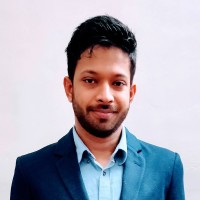
\includegraphics[width = 4cm]{pic}}; 
    % if necessary the picture may be moved by changing the at (coordinates)
    % width defines the 'zoom' of the picture
\end{tikzpicture}
}
\end{tabularx}

%-----EDUCATION----------------------------------------------------------------
\section{\textbf{Education}}

  \CVSubHeadingListStart
%    \CVSubheading % Example
%      {Degree Achieved}{Years of Study}
%      {Institution of Study}{Where it is located}
    \CVSubheading
      {{\textbf{Master of Science} $|$ {\small{INFOTECH}}}}{Oct. 2018 -- Ongoing}
      {University of Stuttgart}{Stuttgart, Germany}
      \item{\textbf{Master Thesis:} Error Detection in Unmanned Aerial Vehicle using Machine Learning and Deep Learning.}
    %   \item{\textbf{Relevent Courses:} Deep Learning \| Service Computing \| Human-Computer Interaction Lab. \| Data Mining and Data Warehousing \| Advance Software Testing \& Analysis}
    
    \vspace{3pt}

    \CVSubheading
      {{\textbf{Bachelor of Technology} $|$ {\small{Electronics and Communication Engineering}}}}{Aug. 2012 -- May 2016} {Maulana Abul Kalam Azad University of Technology}{West Bengal, India}
      \item{\textbf{Bachelor Thesis:} Design of Digital FIR Filters using meta-heuristic Optimization Algorithms.}\hspace{2pt}{\href{https://github.com/Niloy-Chakraborty/G_best-Guided-Cuckoo-Search-Algorithm}{\faGithub}}
    
  \CVSubHeadingListEnd



%-----WORK EXPERIENCE----------------------------------------------------------


\section{\textbf{Work Experience}}

  \CVSubHeadingListStart
  
     \CVSubheading
      {Working Student in Data Science}{Oct 2020 -- Ongoing}
      {\textbf{Koena tec GmbH}}{Stuttgart, Germany}
      \CVItemListStart
        \CVItem{Data collection and building data \textbf{pre-processing pipeline}.}
        \CVItem{Implemented Coffee Order detection Classification using \textbf{Random Forest, SVM} and predicting future consumption using \textbf{Composite LSTM Autoencoder}.}
        \CVItem{Deployed the model in the cloud using \textbf{Docker}.}

        \CVItemListEnd
    \vspace{0.2cm}
    \CVSubheading
      {Intern in Predictive Analytics}{Mar 2020 -- Aug 2020}
      {\textbf{Robert Bosch GmbH}}{Stuttgart, Germany}
      \CVItemListStart
        \CVItem{\textbf{Log data parsing} and \textbf{Process Mining} of the in-house Software (myMBR) to bring insights from data.}
        \CVItem{\textbf{User Journey analysis} and Visualization using \textbf{Power BI} and finding the bottlenecks of the software.}
        \CVItem{Development of Purchase Order Denial Model using \textbf{Random Forest Algorithm}.}
        
    \CVItemListEnd
    \vspace{0.2cm}

    \CVSubheading
      {Scientific Research Assistant}{Feb 2019 -- Dec 2019}
      {\textbf{Fraunhofer IAO}}{Stuttgart, Germany}
      \CVItemListStart
        \CVItem{Collection and analysis of smart meter dataset.}
        \CVItem{\textbf{Time-series stream clustering} using \textbf{Kmeans} and \textbf{Hierarchical Clustering} algorithms for finding correlation in the different subscription categories.}
        \CVItem{Building Visualization dashboard for realtime streaming using \textbf{Flask} and \textbf{Plotly.js}.}
      \CVItemListEnd
    \vspace{0.2cm}
  
    \CVSubheading
      {Scientific Research Assistant}{July 2019 -- Dec 2019}
      {\textbf{IAAS-University of Stuttgart}}{Stuttgart, Germany}
      \CVItemListStart
        \CVItem{Building data pipeline for smart data-center, including \textbf{data staging area}, \textbf{message queuing} using \textbf{Rabbit-MQ} .}
        \CVItem{Developed \textbf{real-time data monitoring} dashboard using \textbf{Chronograf}.}

    \CVItemListEnd
    \vspace{0.2cm}

    
    \CVSubheading
      {System Engineer}{Jul 2017  -- Sep 2018}
      {\textbf{AI For Networks Lab, Tata Consultancy Services Limited}}{Hyderabad ,India}
      \CVItemListStart
        \CVItem{Developed \textbf{IP Network Anomaly Detection} tool using \textbf{LSTM} and associated Web-API using \textbf{Python}, \textbf{Flask}, \textbf{HTML5}, \textbf{CSS}, and \textbf{JavaScript}.}
        \CVItem{Implemented Deep Learning based \textbf{KPI prediction} using \textbf{Conv-GRU} algorithm.}
        \CVItem{Implemented \textbf{Defect category classification} for defect tracking system using \textbf{Random Forest} Algorithm.}
    \CVItemListEnd
  \CVSubHeadingListEnd

\section{\textbf{Skills}}
 \begin{itemize}[noitemsep]
 
    \item{\textbf{Language:} English (Fluent), German (Elementary)}
    
     \item{\textbf{Scripting/Programming Language:} Python, MATLAB, Java, JavaScript, C, VBA}
     
    \item{\textbf{ML Libraries/Frameworks:} Tensorflow, Keras, Pandas, Scikit-learn, Numpy, Scipy, Matplotlib}
     
     \item{\textbf{Databases:} MongoDB, MySql, SqLite}
     \item{\textbf{Web Technologies/Frameworks:} HTML5, CSS, JSON, Node.js, Flask}
     \item{\textbf{Automation:} Apache Airflow, Jenkins, Docker}
     \item{\textbf{Others:} Git, Agile, Confluence, PyCharm, Jupyter Notebook, Eclipse}
     
    

  
 \end{itemize}

%-----PROJECTS AND RESEARCH----------------------------------------------------

\section{\textbf{Projects and Research}\hspace{3pt}{\href{https://github.com/Niloy-Chakraborty/}{\faGithub}}}
  \CVSubHeadingListStart
        \CVSubheading
      {Human Attention Prediction for Webpages}{}
      {Stuttgart, Germany}{\href{https://github.com/Niloy-Chakraborty/Webpage_Saliency_Prediction}{\faGithub}}
      \CVItemListStart
        \CVItem{A study of eye tracking attention dataset for websites using FiWi dataset (only 149 images).}
        
       \CVItem{A 2 stage Transfer Learning process was used to to predict the human attention map using SVM and VGG 16 based Fully connected CNN with skip connections.}
       \CVItem{The results were compared with the top saliency models like SALICON, Deep Gaze 2.}
    \CVItemListEnd
    
            \CVSubheading
      {My Smart Home Garden}{}
      {Stuttgart, Germany}{\href{https://github.com/Niloy-Chakraborty/Smart-Gardening}{\faGithub}}
      \CVItemListStart
        \CVItem{A Telegram bot was built to automate gardening system (Watering, Lighting, and Plant Identification)}
        \CVItem{Cloud based data storage pipeline and dashboard for sensor and weather data was built.}
        \CVItem{An AI planning model was developed for automatic watering and lighting.} 
        \CVItem{CNN based plant name and health identification models were developed.}
    \CVItemListEnd
    
        \CVSubheading
      {Real Time Data Monitoring System}{}
      {Stuttgart, Germany}{\href{https://github.com/Niloy-Chakraborty/Real-Time-Data-Monitoring-System}{\faGithub}}
      \CVItemListStart
        \CVItem{This project shows an end-to-end data flow pipeline via RabbitMQ and InfluxDB for sensor/ network KPI data.}
        \CVItem{The data can be visualized via Chronograf in Real-Time for further analysis.}

    \CVItemListEnd
    
    \CVSubheading
      {Time Series Stream Clustering for Smart Meter Data}{}
      {Stuttgart, Germany}{\href{https://github.com/Niloy-Chakraborty/Time-Series_Clustering_on_London_Smart_Meter_Dataset}{\faGithub}}
      \CVItemListStart
        \CVItem{Analysis and pre-processing of London Smart Meter sensor dataset. }
        \CVItem{Time-series clustering of the  using K-means, Hierarchical clustering, and Auto encoder.}
 
    \CVItemListEnd
    
    \CVSubheading
      {Model Based Test Driven Development}{}
      {Stuttgart, Germany}{}
      \CVItemListStart
        \CVItem{An approach for developing faster Regression test suites and also in executing multiple test cases with less manual intervention.}
        \CVItem{It uses Finite State Machines for visual representation of test cases.}
        \CVItem{It also has features like tree visualization of the yang files, python code editor for writing test cases , syntax checker, graph editor etc.}
    \CVItemListEnd
    
  \CVSubHeadingListEnd

%-----CONFERENCES AND PRESENTATIONS--------------------------------------------
\begin{comment}
Again the title should have already been enough, but if it is necessary to add
descriptions maintain the consistency from prior sections
\end{comment}

\section{\textbf{Publications}\hspace{3pt}{\href{https://www.researchgate.net/profile/Niloy-Chakraborty}{\faExternalLink}}}

  \CVSubHeadingListStart
%    \CVSubheading % Example
%      {Work Presented}{When}
%      {Occasion}{}
    \CVSubheading
      {IP Network Anomaly Detection using Machine
Learning}{\href{https://ieeexplore.ieee.org/document/9033545}{\faExternalLink}}
      {IEEE Conference Paper (I2CT 2019){}}
      
    \CVSubheading
      {Whale Optimization Algorithm: An Implementation
to design low-pass FIR Filter}{\href{https://ieeexplore.ieee.org/document/8244929}{\faExternalLink}}
      {IEEE Conference Paper (iPACT 2018)}{}
      
    \CVSubheading
      {Design of IIR filter Using Gbest Guided Cuckoo
Search Algorithm}{\href{https://ieeexplore.ieee.org/document/8009573}{\faExternalLink}}
      {IEEE Conference Paper (ICCECE 2016)}{}
          \CVSubheading
      {Design of Higher order FIR Low Pass Filter using
Cuckoo Search Algorithm}{\href{https://ieeexplore.ieee.org/document/7754285}{\faExternalLink}}
      {IEEE Conference Paper (ICCSP 2016)}{}
  \CVSubHeadingListEnd

%-----HONORS AND AWARDS--------------------------------------------------------
\section{\textbf{Honors and Awards}}
 \begin{itemize}[leftmargin=0.5cm, label={}]
    \small{\item{
     \textbf{1. }{Recommended for \textbf{Student @ Bosch} program for Internship performance.} \\
         \textbf{2. }{Best Performer of the Month, and Special Initiative award during my Full time job, for my contribution in the \textbf{R\&D}.}\\
\textbf{3. }{Received Scholarship from \textbf{All India Council for Technical Education} for National Level technical training program.} \\
     \textbf{4. }{Honoured with \textbf{VIDYASHREE} titled award for outstanding performance in the 10th Grade.} \\
     

 

    }}
 \end{itemize}

%-----TEACHING EXPERIENCE------------------------------------------------------
\begin{comment}
Section is here as it applied to my application for positions in academia. 
Remember to tailor the resume for to the position.
\end{comment}

%------------------------------------------------------------------------------
\end{document}